\section{Domain, Range, and End Behavior}

{
    \small
    \begin{tcbraster}[
        raster columns=3,
        colback=white,
        raster equal height,
        raster after skip = 3\baselineskip,
        ]
        \begin{tcolorbox}
            \raggedright
            {\bfseries\itshape Domain.} $x$ values 
            of all the {points on the graph}
            of a function.
        \end{tcolorbox}
        \begin{tcolorbox}
            \raggedright
            {\bfseries\itshape Range.} $y$ values 
            of all the {points on the graph}
            of a function.
        \end{tcolorbox}
        \begin{tcolorbox}
            \raggedright
            {\bfseries\itshape End behavior.} Written like this:
            \renewcommand{\arraystretch}{1.25}
            \begin{tabular}{lll}
                as & $x \rightarrow -\infty$ & $y \rightarrow \text{\fbox{\phantom{999}}}$ \\
                as & $x \rightarrow +\infty$ & $y \rightarrow \text{\fbox{\phantom{999}}}$ \\
            \end{tabular}
        \end{tcolorbox}
    \end{tcbraster}
}

We will explore these interactively
using a {\scshape Desmos} activity
where we will \gap{drag} a point back and forth 
to see what happens to \gap{$x$} and \gap{$y$}.

\begin{myAnnotate}{{Activity}}{Using {Desmos} to slide points on a curve.}[%
    center,
    width=5.5in,
    before skip = 3\baselineskip,
    colbacktitle=black!15,]
    \begin{itemize}[nosep]
        \item Get out your phone---{\itshape mirabile dictu!}
        \item Open a browser to {\ttfamily student.desmos.com}.
            \begin{center}
                \fbox{
\includegraphics[width=3in]{student-desmos-com}}
            \end{center}
        \item Join with this code: {\ttfamily U2MWUS}. (Do not login.)
        \item There are 3 screens in the activity. 
            \begin{center}
                \fbox{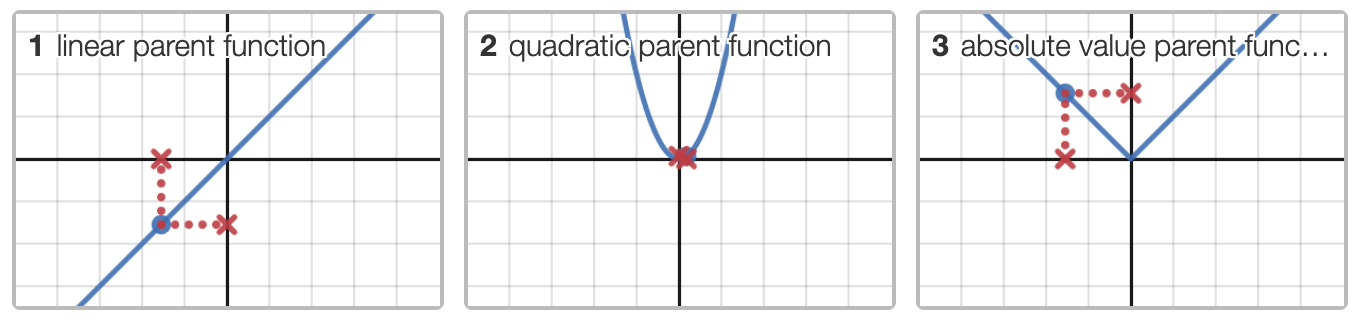
\includegraphics[width=4in]{desmos-activity-screens}}
            \end{center}
        \item Each screen has a draggable point. 
            {\bfseries\itshape Drag them back and forth}.
        \item The following problems relate to these screens.
    \end{itemize}
\end{myAnnotate}

\myWideProblemWithContent[]
{
    {
        \centering\normalsize
        {\scshape Screen 1:}
        \itshape Linear Parent Function: $f(x) = x$
    }
    \tcblower
    \begin{minipage}{0.2\textwidth}
        \centering
        \begin{myTikzpictureGrid}{0.2} {6}{6}
            % \tkzText(13,8){$x - y = 0$}
            \tkzFct[ solid, ultra thick, samples=100, domain=-6:6,]{x}
            \draw[black,thick,fill=black!20] (-5,-5) circle (1.5em);
            \draw[black,thick,fill=black] (-5,-5) circle (0.5em);
        \end{myTikzpictureGrid}
    \end{minipage}
    \hfil
    \begin{minipage}{0.75\textwidth}
        \begin{enumerate}[fullwidth,itemsep=0.3em]
            \item Drag the point back and forth. 
            \item Notice the $x$- and $y$-coordinates projected onto the axes. 
            \item {\bfseries\itshape Domain.} 
                As you watch the $x$-coordinates on the $x$-axis,
                you can see the domain is \gap{all real numbers.}
            \item {\bfseries\itshape Range.} 
                As you watch the $y$-coordinates on the $y$-axis,
                you can see the range is \gap{all real numbers.}
            \item {\bfseries\itshape Left End Behavior.}\\
                As you drag the point to the left
                $x \rightarrow \bm{-}\infty$.
                What happens to the $y$-coordinate?
                The $y$-coordinate moves \gap{down}.
            \item {\bfseries\itshape Right End Behavior.}\\
                As you drag the point to the right,
                $x \rightarrow \bm{+}\infty$.
                What happens to the $y$-coordinate?
                The $y$-coordinate moves \gap{up}.
            \end{enumerate}
    \end{minipage}
}

\myWideProblemWithContent[]
{
    {
        \centering\normalsize
        {\scshape Screen 2:}
        \itshape Quadratic Parent Function: $f(x) = x^2$
    }
    \tcblower
    \begin{minipage}{0.2\textwidth}
        \centering
        \begin{myTikzpictureGrid}{0.2} {6}{6}
            % \tkzText(13,8){$x - y = 0$}
            \tkzFct[ solid, ultra thick, samples=100, domain=-6:6,]{x**2}
            \draw[black,thick,fill=black!20] (-2,4) circle (1.5em);
            \draw[black,thick,fill=black] (-2,4) circle (0.5em);
        \end{myTikzpictureGrid}
    \end{minipage}
    \hfil
    \begin{minipage}{0.75\textwidth}
        \begin{enumerate}[fullwidth,itemsep=0.3em]
            \item {\bfseries\itshape Domain.} 
                The domain is \gap{all real numbers.}
            \item {\bfseries\itshape Range.} 
                The range is \gap{$y \ge 0$}.
            \item {\bfseries\itshape Left End Behavior.}\\
                As $x \rightarrow -\infty$ (to the left),
                $y$ moves \gap{up} ($y \rightarrow$ \gap{$+\infty$}).
            \item {\bfseries\itshape Right End Behavior.}\\
                As $x \rightarrow +\infty$ (to the right),
                $y$ \gap{up} ($y \rightarrow$ \gap{$+\infty$}).
        \end{enumerate}
    \end{minipage}
}


\myWideProblemWithContent[]
{
    {
        \centering\normalsize
        {\scshape Screen 3:}
        \itshape Absolute Value Parent Function: $f(x) = |x|$
    }
    \tcblower
    \begin{minipage}{0.2\textwidth}
        \centering
        \begin{myTikzpictureGrid}{0.2} {6}{6}
            % \tkzText(13,8){$x - y = 0$}
            \tkzFct[ solid, ultra thick, samples=100, domain=-6:6,]{abs(x)}
            \draw[black,thick,fill=black!20] (4,4) circle (1.5em);
            \draw[black,thick,fill=black] (4,4) circle (0.5em);
        \end{myTikzpictureGrid}
    \end{minipage}
    \hfil
    \begin{minipage}{0.75\textwidth}
        \begin{enumerate}[fullwidth,itemsep=0.2em,]
            \item {\bfseries\itshape Domain.} 
                The domain is \gap{all real numbers.}
            \item {\bfseries\itshape Range.} 
                The range is \gap{$y \ge 0$}.
            \item {\bfseries\itshape Left End Behavior.} 
                As $x \rightarrow -\infty$,
                $y \rightarrow$ \gap{$+\infty$}.
            \item {\bfseries\itshape Right End Behavior.} 
                As $x \rightarrow +\infty$,
                $y \rightarrow$ \gap{$+\infty$}.
        \end{enumerate}
    \end{minipage}
}

